\documentclass[pre,preprint]{revtex4-1}

% preamble:
\usepackage{appendix}
\usepackage{outline}
\usepackage{amsmath}    % need for subequations
\usepackage{graphicx}   % need for figures
\usepackage{verbatim}   % useful for program listings
\usepackage{color}      % use if color is used in text
\usepackage{subfigure}  % use for side-by-side figures
\usepackage{hyperref}   % use for hypertext links, including those to external documents and URLs
\raggedbottom           % don't add extra vertical space
\begin{comment}
\pagestyle{empty}       % use if page numbers not wanted
\end{comment}




\begin{document}

\title{Effective viscosity of compliant filament networks with cross-link slip}
\author{William McFadden}
\affiliation{University of Chicago, Biophysical Sciences Program, Chicago, IL 60615}

\date{1 January 2015}

\begin{abstract}
We describe a theoretical model for long timescale rates of deformation in semi-flexible filament networks with transient cross-links.  We have addressed the problem using a mechanical picture where cross-linked filaments are allowed to slip past one another in a linear drag-like manner.  This model gives predictions for the long timescale effective viscosity of the medium that depends on network architecture and effective drag coefficient between filaments.  We use computational simulations to predict deviations from purely viscous creep when networks undergo large strains that drive them into anisotropic configurations.  Interestingly, under certain conditions, we find a phase of long-lived sub-linear creep, suggesting that our simple model can account for the broad relaxation timescales measured in biopolymer rheological experiments.
\end{abstract}

\maketitle


\tableofcontents


















\section{Introduction}

Cross-linked networks of semi-flexible polymers are a class of materials with poorly understood but highly interesting properties.  They have been a subject of great interest for many years largely due to their biological importance forming structural components of cells\cite{cellmech_review1,cellmech_review2}.  However, early studies of {\em in vitro} reconstitutions of semi-flexible polymer networks soon revealed novel, nonlinear rheology, spurring further interest from materials scientists\cite{megareview}.  

After many years of study, much of the intermediate timescale behavior (between 1-1000 seconds) of these networks has been well-described theoretically in terms of purely elastic mechanical responses.  However, on longer timescales, the network's elastic resistance begins to give way to a viscous relaxation of stored stress.   It is important to understand the mechanism behind this long timescale behavior of cross-linked polymer networks both for understanding their novel material properties as well as understanding how this effect may govern physiologically important cellular processes\cite{cell_rheo}.

For {\em in vitro} reconstitutions, this viscous relaxation is thought to be a result of the transient unbinding and rebinding of intermolecular cross-links\cite{rheo_crosslinksmatter,theo_crosslinkslip1}. Despite this mechanism being suspected as the source of the viscous stress relaxation, there is still no clear understanding of the particular manner in which these local relaxations of network connectivity would give rise to a global viscous relaxation.  In our work, we wish to expand upon a micro-mechanical picture of cross-linked semi-flexible polymer networks to incorporate slippage of cross-links over longer timescales.  


\subsection{Short Timescale Mechanics of Cross-linked Filament Networks}

When first tested, {\em in vitro} reconstitutions of intracellular biopolymers were quickly recognized as an interesting viscoelastic material \cite{rheo_actingel}.  These networks exhibited strikingly different elastic behavior compared to the already well-understood flexible polymer gels \cite{rheo_bench}.  This complexity of experimental observation drove a surge in both experimental and theoretical studies of semi-flexible networks.  For a comprehensive review of this field we recommend \cite{megareview}, but we will shortly repeat some important milestones here.

\subsubsection{Theories of Semi-flexible Filament Networks}
 
Diversity and discrepancy in observations led a drive toward systematic {\em in vitro} experimental explorations of the rheology of cross-linked semi-flexible polymer networks at short timescales.  In studies with rigid irreversibly cross-links, it was found that changes could lead to remarkably different elastic moduli, suggesting distinct phases of mechanical response \cite{rheo_marge}.  These discoveries in turn begat theoretical work on the basic implications of the semi-flexible nature of filaments on network mechanics.  

Prior work on the basic physics of individual semi-flexible polymers \cite{mol_wlc,theo_doi_ed}, and comprehensive theories of semi-flexible filament solutions, \cite{theo_morse} laid a groundwork for theoretical considerations of cross-linked networks. Beginning with the so-called "mikado model" descriptions\cite{theo_hlm,theo_hlm2}, it was determined that there should exist a minimum rigidity percolation threshold, and that the connectivity of the network determined whether the mechanical response was dominated by non-affine bending or affine stretching of filaments.   Continuing to more explicit theories\cite{theo_best}, the mechanics of rigidly cross-linked networks were shown to be well-described in terms of purely elastic stretching of filaments between cross-linked points.  

\subsubsection{Incorporating Effects of Cross-link Compliance}

Despite the success of the theory for rigid cross-links, early studies showed surprising qualitative differences in mechanical response could be traced to differences in the chosen cross-linker\cite{rheo_crosslinkcompare,rheo_crosslinkreview}.  In addition, many studies using more compliant cross-linkers showed that cross-linker compliance could give rise to different nonlinear rheological properties on short timescales\cite{rheo_crosslink_nonlin1,rheo_crosslink_nonlin2,rheo_crosslink_nonlin3,rheo_crosslink_notactin}. Making matters even more complicated, ongoing research has begun to uncover added complexity from more highly complex issues such as filament bundling\cite{theo_crosslinkslip2,model_massive}and the effects of active cross-linking by molecular motors\cite{rheo_active}.

While theorists have built a number of largely successful models that help characterize different aspects of the cross-link dominated response\cite{theo_nonaffine2,theo_floppy,theo_crosslinknonlinear}, the diversity of behaviors of these networks makes a precise yet general theory more difficult.

\subsection{Long Timescale Stress Relaxation from Transient Cross-link Unbinding}

At long timescales, the purely elastic behavior of cross-linked networks gives way to fluid-like stress relaxation. Additionally, fluid-like flows have been observed in a number of cellular processes\cite{cellmech_flows,cellmech_flows2,cellmech_flows3,rheo_fluid,rheo_fluid2,cell_rheo_exp}.  In {\em in vitro} studies, long timescale creep behaviors are thought to arise predominantly from the transient nature of binding for most biologically relevant cross-linkers\cite{rheo_crosslinkslip1,rheo_crosslinkslip2,rheo_crosslinkslip3,rheo_nonaffine}.  While the importance of cross-link dynamics in determining the mechanical response of semi-flexible polymer networks has been known for at least 20 years\cite{rheo_crosslinksmatter}, there is still a gap in our understanding of how microscopic cross-link unbinding relates to viscous flows. 

\subsubsection{Models of Stress Relaxation with Transient Cross-links}

The dependence of network rheology on cross-link unbinding is an active subject of theoretical research\cite{theo_crosslinkslip2}.  

Many theoretical methods have sought to model cross-link binding and unbinding directly\cite{theo_crosslinkslip1,theo_crosslinkslip2}, and previous modeling work often take cross-links as extended springlike structures \cite{model_taeyoon} separate from the main semi-flexible filament constituents.  \cite{rheo_crosslinkslip2}
\cite{theo_crosslinkslip3}

\subsubsection{Novelty of Cross-link Slip Approach}


In our current work, we simplify our approach to coarse-grained filaments which are able to slide past each other as molecular bonds form and rupture, akin to coarse-grained models of molecular friction\cite{theo_friction,theo_frictionSam,theo_molefric}.  This drag-like coupling has been shown to be an adequate approximation in the case of ionic cross-linking of actin\cite{mol_fric,theo_hydroish2}, and can be found in the theoretical basis of force-velocity curves for myosin bound filaments\cite{theo_frictionShila}. We propose that it will form a suitable bulk approximation in the presence of super molecular cross-links as well.

Importantly, this simplification allows us to extend our single polymer models to dynamical systems of larger network models for direct comparison between theory and modeling results.  This level of coarse graining will therefore make it easier to understand classes of behavior for varying compositions of cross-linked filament networks.  In addition, it allows us to compute a new class of numerical simulations efficiently, which gives us concrete predictions for behaviors in widely different networks with measurable dependencies on molecular details.



































\section{Explanation of Model}

\subsection{Composite Cross-link \& Filament Representation}
We consider individual semi-flexible polymers as chains of springs of relaxed length $l_s$, whose orientations are linearly coupled to their neighbors. Filaments can be represented as a sequence of nodes with positions $\mathbf{x_i}$ and nearest neighbor interactions of the form

\begin{equation}
|F_{i,i+1}|_{\parallel} = -\mu\cdot\frac{|\mathbf{x_{i+1}}-\mathbf{x_i}|-l_s}{l_s} 
\end{equation}

\begin{equation}
|F_{i,i+2}|_{\perp} = -\frac{\kappa}{l_s^2}\cdot acos\left (\frac{\mathbf{x_{i+2}}-\mathbf{x_{i+1}}}{|\mathbf{x_{i+2}}-\mathbf{x_{i+1}}|} \cdot\frac{\mathbf{x_{i+1}}-\mathbf{x_i}}{|\mathbf{x_{i+1}}-\mathbf{x_i}|} \right ) 
\end{equation}

This is essentially a discretized equivalent to a model of filaments with separable extensional and bending moduli like the type in \cite{theo_hlm} with a potential defined by
\begin{equation}
{\cal H} =\frac{1}{2}\kappa \int ds(\nabla^2\mathbf{u})^2 + \frac{1}{2}\mu \int ds \left ( \frac{dl(s) }{ds} \right )^2
\end{equation}

where, $\mu$ represents an extensional modulus of a filament, and $\kappa$ represents a bending modulus.   

Here, the extensional and bending moduli are taken as composite quantities related to both filament and cross-linker compliance in a manner similar to a recently proposed effective medium theory\cite{theo_crosslinknonlinear}.  We provide a molecular level derivation of this composite compliance in Appendix \ref{app:compos}, but for now we wish to highlight the main features.  

In the limit of highly rigid cross-links and flexible filaments, our model clearly reduces to the pure semi-flexible filament models of \cite{theo_hlm,theo_hlm2}.  In the opposite regime of nearly rigid filaments and highly flexible cross links, our method is still largely similar to the model of \cite{theo_crosslinknonlinear} in small strain regimes before any nonlinear cross link stiffening.  However, in departure from those models, the magnitude of the force on interior cross-links in our model is still the same as those on the exterior.  This is a simplification of the varying levels of strain that would actually be present in these cross-linkers, but we choose to ignore the slight variation in favor of an approximate, universal approach.  Finally, in the event that the induced strain of the filament and the cross-linker are of comparable scales, our composite stiffness can be expressed by the approximation $huh$ as we shown in Appendix \ref{app:compos}.

In our simulations we explore the role that nonlinear stiffening of filaments or cross linkers would play, and what complications arise.

\subsection{2D Network Formation}

We choose to focus our attention on 2D networks both for their tractability as well as their relevance in the quasi-2D cytoskeletal cortex of many mammalian cells\cite{cellmech_flows}.  In addition, recent developments in 2D {\em in vitro} systems\cite{rheo_2D1,rheo_2D2}, make 2D models all the more interesting as a renewed focus of study.

We are using a minimal network (Mikado model) of connected unstressed linear filaments in a rectangular 2D domain.  We generate 2D networks of these semi-flexible filaments by laying down straight lines of length, $L$, with random position and orientation. We then assume that some fixed fraction of overlapping filaments become cross-linked (defined in \ref{exp_drag}) at their point of overlap.

Although real cytoskeletal networks may form with non-negligible anisotropy, we choose to focus our attention on isotropically initialized networks for simplicity.  We define the density using the average distance between cross-links along a filament, $l_c$. A simple geometrical argument can be used to derive the number of filaments filling a domain as a function of $L$ and $l_c$\cite{theo_hlm}.  However, for our purposes we take the approximation that the number of filaments needed to tile a rectangular domain of size $W \times H$  is $2WH/Ll_c$, and that the length density is therefore $1/l_c$. 

In the absence of cross-link slip, we expect the network to comprise a connected solid with a well defined elastic modulus\cite{theo_hlm,theo_hlm2}.  These networks are only well-connected when the ratio of filament length to intercrosslink spacing, $L/l_c$ is greater than $\sim 6$.  Near this percolation threshold, there are only locally connected domains, and discussions of global network properties becomes less reasonable.  Additionally, as the filament density is increased beyond this point, there is another transition between non-affine bending and affine stretching of filaments, which changes the dominating term of the network's elastic modulus.



\subsection{Drag-like Coupling Between Overlapping Filaments}
\label{exp_drag}
In departure from the previous models, we wish to incorporate relaxation of the network's stored stress by letting the attachment points slip.  We do this by replacing the fixed with a drag-like coupling between filaments.
\begin{equation}
\mathbf{F_{drag}} = \xi \cdot \int ds \: (\mathbf{v(s)}-\mathbf{v_0(s)}) \: f(s)
\end{equation}

Where $f(s)$ represents the locational distribution of cross-link points (equal to 1 at locations of cross-links and 0 elsewhere).  This model assumes a linear relation between applied force and the velocity difference between attached filaments.  Obviously, non-linearities can arise in the presence of force dependent detachment kinetics as well as non-linear force extension of cross-links.  In particular, we address non-linear effects of stress induced unbinding in Appendix \ref{app:drag}.  Assuming inhomogeneities from non-linear effects are of second order, the motion for the entire network is governed by a dynamical equation of the form

\begin{equation}
\label{eqn:syst}
\int ds \: (\mathbf{\zeta v_i(s)} + \xi \sum _j(\mathbf{v_i(s)}-\mathbf{v_j(s)}) \: p_{ij}(s))= \nabla {\cal H}_i
\end{equation}

Here, the first term in the integral is the filament's intrinsic drag through its embedding fluid, $\zeta$, while the second comes from the drag-like coupling between filaments, $\xi$.  


\subsection{System of Equations for Applied Stress}
We model our full network as a coupled system of differential equations satisfying \ref{eqn:syst}.  Although the general mechanical response of this system may be very complex, we wish to focus our attention on low frequency deformations and the steady-state creep response of the system to an applied stress.  To do this we introduce a fixed stress, $\sigma$ along the midline of our domain.  This stress will point in the direction, $\mathbf{\hat{u}}$, producing either shear ($\mathbf{\hat{u}}=\mathbf{\hat{x}}$) or extensional ($\mathbf{\hat{u}}=\mathbf{\hat{y}}$) stress.

Finally, we add a 0 velocity constraint at the far edges of our domain of interest.  We assume that our network is in the "dry," low Reynold's number limit, where inertial effects are so small that we can equate our total force to 0.  Therefore, we have a dynamical system of wormlike chain filaments satisfying 

\begin{equation}
\int ds \: (\zeta\mathbf{v_i(s)} + \xi \sum _j(\mathbf{v_i(s)}-\mathbf{v_j(s)}) \: p_{ij}(s)) = \nabla {\cal H}_i + \sigma\mathbf{\hat{u}}\cdot\delta(x-D)
\end{equation}

subject to constraints such that $\mathbf{v_i(x)}$ is 0 with $x=0$.  This results in an implicit differential equation for filament segments which can be discretized and integrated in time to produce a solution for the motion of the system.


\subsection{Computational Simulation Method}

We tested our analytical conclusions on a computational model.  The technical details of the model can be found in the Appendix, but we summarize the main modeling points here.

We discretize the filaments such that the equations of motion becomes a coupled system of equations for the velocities of filament endpoints, $\mathbf{x}$.  The drag-like force between overlapping filaments results in a coupling of the velocities of endpoints.  

\begin{equation}
\mathbf{A \cdot \dot x} = \mathbf{f(x)}
\end{equation}

where $\mathbf{A }$ represents a coupling matrix between endpoints of filaments that overlap, and $\mathbf{f(x)}$ is the spring force between pairs of filament segment endpoints.  We can then numerically integrate this system of equations to find the time evolution of the positions of all filament endpoints.

We generate a network by laying down filaments with random position and orientation within a domain of size $2D$ by $D$ with periodic boundaries.  The external stress (shear or extensional/compressional) is applied to all filament endpoints falling within a fixed x-distance from the center of the domain.  Finally, filament endpoints falling within a fixed x-distance from the edges of the domain are constrained to be nonmoving.

\begin{figure}[h!]
\centering
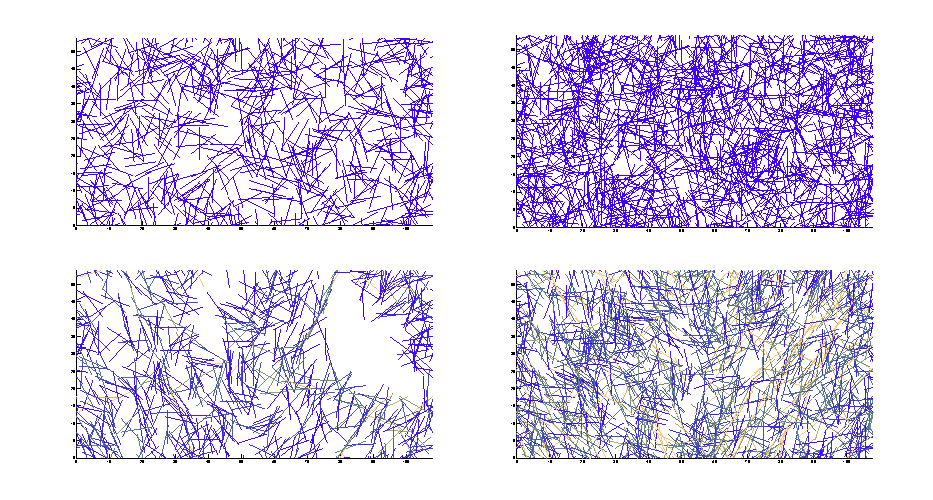
\includegraphics[width=\hsize]{network_def}
\caption{\label{fig:sim}Two Simulation setups with $L=9 \mu m, D = 54 \mu m$ before and after 1000s of applied stress. a) low density $l_c=2 \mu m$, b) moderate density $l_c=1 \mu m$ }
\end{figure}

The nominal units for length, force, and time are $\mu m$, nN, and s, respectively.  We explored parameters space around an estimate of biologically relevant parameter values, given in Table X. 

For computational simplicity in these models, unless otherwise mentioned we assume that the bending rigidity, $\kappa$, is infinite. This allows us to model filaments as non-bending springs of rest length, $L$, and spring modulus $\mu$.  In the appendix, we show that our result is not significantly different from the result for semi-flexible polymers.































\section{Modes of deformation under Shear Stress}


\subsection{Low Strain Approximation of Effective Viscosity}
We would like to begin with a calculation of a low-strain estimate of the effective viscosity for a network described by our model.  We carry this out by assuming we have applied a constant stress along a transect of the network.  With moderate stresses, we assume the network reaches a steady state affine creep. In this situation, we would find that the stress in the network exactly balances the sum of the drag-like forces from cross-link slip.  So for any transect of length D, we have a force balance equation.

\begin{equation}
\mathbf{\sigma} = \frac{1}{D}\sum_{filaments}\: \sum_{crosslinks}\xi \cdot (\mathbf{v_i}-\mathbf{v_0})
\end{equation}

where $\mathbf{v_i(s)}-\mathbf{v_j(s)}$ is the difference between the velocity of a filament at it's cross-link point and the velocity of the filament to which it is a attached. We can convert the sum over cross-links to an integral over the length using the average density of cross-links, $1/l_c$ and invoking the assumption of (linear order) affine strain rate, $\mathbf{v_i}-\mathbf{v_0}=\dot \gamma x$. This results in

\begin{multline}
\mathbf{\sigma} =  \frac{1}{D}\sum_{filaments}\:  \xi \cdot \int_0^L ds \: (\mathbf{v(s)}-\mathbf{v_0(s)}) \:\frac{1}{l_c} \\
 = \sum_{filaments}\:  \frac{\xi \dot \gamma L}{l_c} \cos \theta \cdot (x_l + \frac{L}{2} \cos \theta)
\end{multline}

Here we have introduced the variables $x_l$, and $\theta$ to describe the leftmost endpoint and the angular orientation of a given filament respectively.  Next, to perform the sum over all filaments we wish to convert this to an integral over all orientations and endpoints that intersect our line of stress. We assume for simplicity that filament stretch and filament alignment are negligible in this low strain approximation.  Therefore, the max distance for the leftmost endpoint is the length of a filament, L, and the maximum angle as a function of endpoint is $\arccos(x_l/L)$.  The linear density of endpoints is the constant $D/l_cL$ so our integrals can be rewritten as this density over $x_l$ and $\theta$ between our maximum and minimum allowed bounds.

\begin{equation}
\mathbf{\sigma} =  \frac{1}{D} \int_0^L dx_l \int_{-\arccos (\frac{x_l}{L})}^{\arccos (\frac{x_l}{L})}\frac{d\theta}{\pi} \frac{\xi \dot \gamma L}{l_c} \cdot \frac{D}{Ll_c}\cdot (x_l \cos \theta + \frac{L}{2} cos^2\theta)
\end{equation}

Carrying out the integrals and correcting for dangling filament ends leaves us with a relation between stress and strain rate.

\begin{equation}
\mathbf{\sigma} = \frac{(L-2l_c)^2 \xi}{4\pi l_c^2} \dot \gamma 
\end{equation}

We recognize the constant of proportionality between stress and strain rate as a viscosity.  Therefore, our approximation for the effective viscosity, $\eta_{eff}$, at steady state creep in this low strain limit is

\begin{equation}
\label{lin_eqn}
\eta_{eff} = \frac{(L-2l_c)^2 \xi}{4\pi l_c^2} .
\end{equation}

With moderate strains ($\gamma<0.2$), our computational simulations show that in the high density limit, our theoretical approximation from Eqn \ref{lin_eqn} is highly accurate at explaining the network behavior.  Aside from a geometrical factor, our approximation is valid for both shear and extensional stresses applied to the network.

As the density of the network approaches the breakdown limit, the effective viscosity diverges from our expected value.  At the low connectivity limit, our expected viscosity goes to 0, but the medium viscosity begins to take over as we cross the percolation threshold.  
\begin{figure}[h!]
\centering
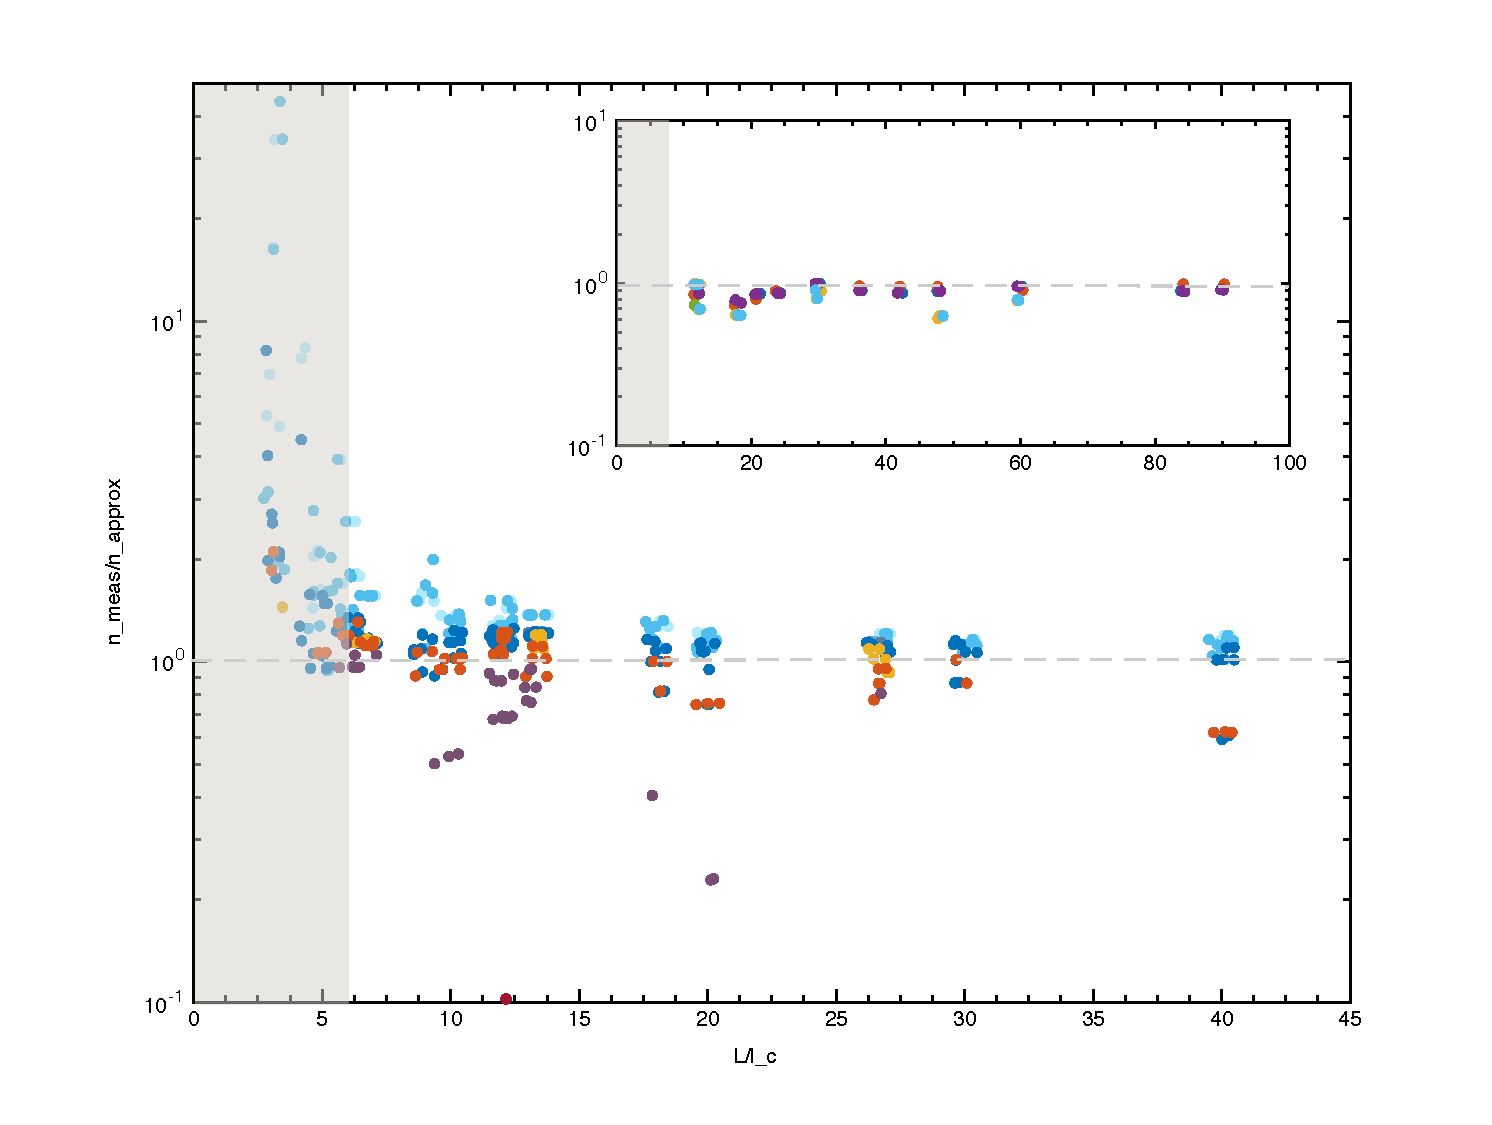
\includegraphics[width=\hsize]{eff_vic_master}
\caption{\label{fig:effvic}Ratio of effective viscosity measured by shear simulation to predicted effective viscosity as a function of connectivity, $L/l_c$. Inset: Same measurement for extensional simulations }
\end{figure}

In addition to changing the architecture and effective drag coefficient, we also validated the generality of our approximation by varying simulation size, medium viscosity, filament stiffness, and applied stress.  We were able to find a slight trend that depended on filament stiffness as indicated in the difference between blue and red data points in Figure \ref{fig:effvic}.  This deviation from our approximation manifested itself more strongly when filaments were highly compliant, and we therefore interpret this as a higher order manifestation of the strain induced reordering of our networks which we focus on in the next section.



\subsection{Effects from Large Strain}

Large scale reorientation of cross-linked filaments under strain is a subject of active research at the moment [Sayantan].  Therefore, we wished to use our computational approach to extend our understanding of generic filament networks in the regime of shear induced anisotropy.  Because we allowed variation in both the extensibility of individual filaments and the drag-like coupling between filaments, we found that we could induce reordering from high strain via either large filament compliance or large slip (or both).  

In Figure \ref{fig:shear_modes}, we illustrate the four stereotyped phases of the general mechanical behavior that we observed in our networks.  A deforming network typically undergoes a rapid filament stretching, a slower relaxation of stretched constraints, a phase of cross-link slippage, and an eventual alignment and breakdown of network connectivity.

\begin{figure}[h!]
\centering
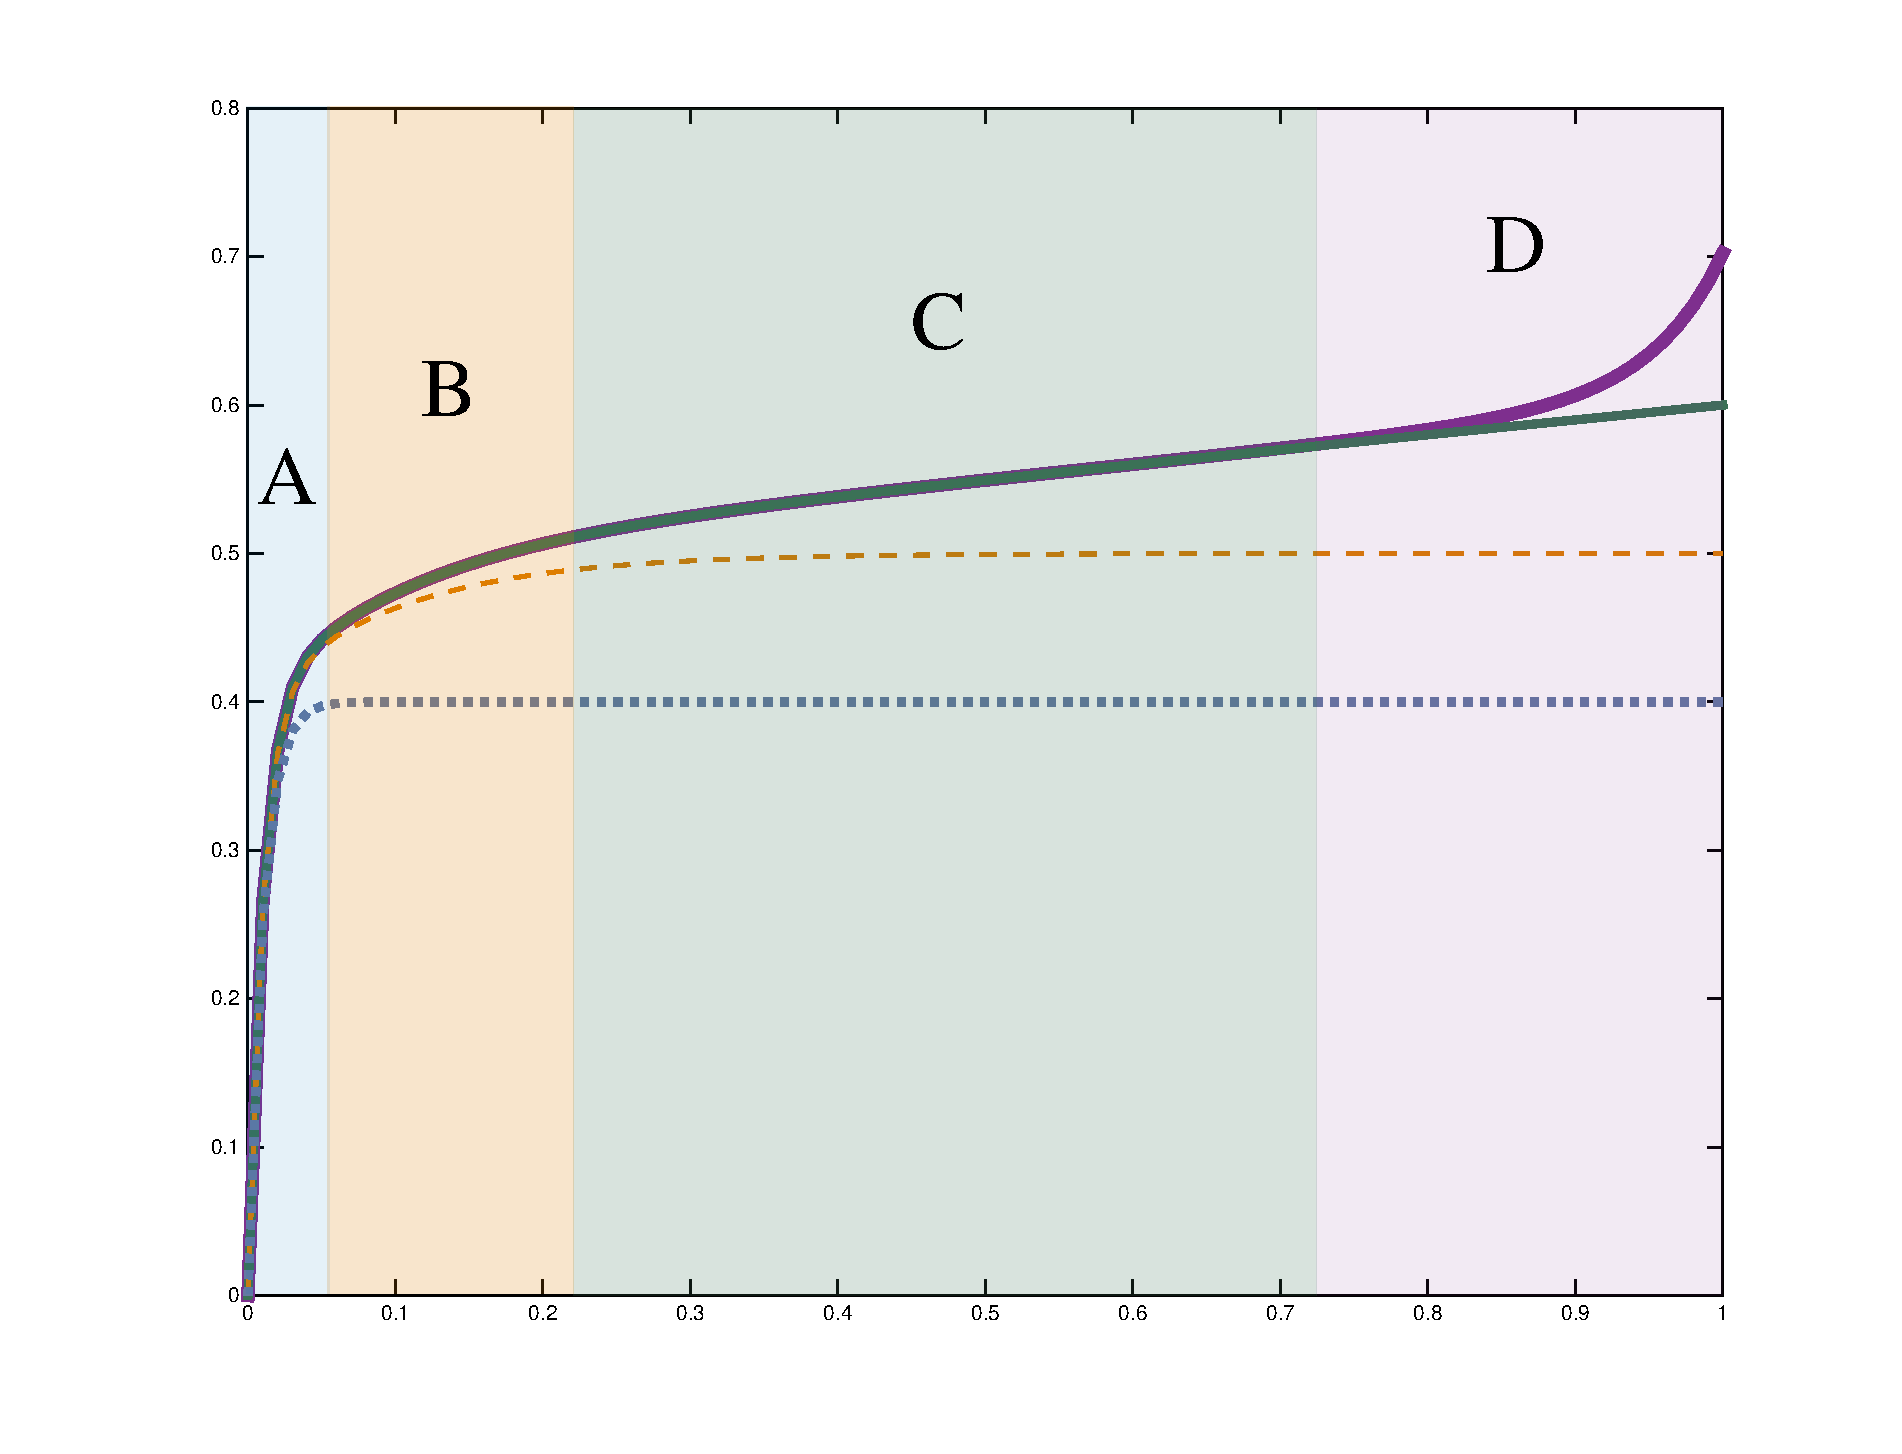
\includegraphics[width=\hsize]{shear_modes}
\caption{\label{fig:shear_modes}Schematic of the general creep response of compliant filament networks illustrating the 4 phases of deformation: a) rapid mechanical response, b) combination of slow filament stretching and cross-link slip, c) cross-link slip dominated, d) network tearing from filament alignment.}
\end{figure}

However, it isn't immediately clear how large these components of the strain will be or over what timescale they might take effect.  For simulation conditions where the filaments are highly rigid, there many be no significant stretching of filaments and the system may enter immediately into the cross-link slippage phase.  For simulations with very high cross-link slip, the network may almost immediately align and tear apart.

To better illustrate to what extent and over what timescale each phase dominates the system behavior, we next aim to determine the dependence of these effects on the microscopic parameters of our model.  As the implications for each phase are quite different, we address each case separately.

\subsubsection{Phase B: Transient Softening from Slow Filament Stretch}
\label{sec:compliant}
In general, filament stretch plays a part in two separate mechanical responses.  In the first response, immediately after the application of an external stress, we see a rapid stretching and compression of filaments (Phase A). This phase corresponds to the elastic relaxation of filament degrees of freedom allowed in the irreversibly cross linked case such as \cite{theo_hlm,theo_hlm2}.  

Perhaps more interestingly, in the presence of cross-link slip, the interplay between filament stretching and cross-link slip gives rise to a second phase that deviates from both purely elastic and purely viscous behavior.  During the first phase, filaments underwent large-scale dilation or contraction depending on their orientation relative to the direction of shear.  However, some portion of the filament is still "under-stretched" due to local constraints from cross-links.  Filaments are able to stretch farther as constraints from the cross-linking points slip.  As cross-link slip allows these constraints to be removed, the filament is able to store more energy, leading to an apparent viscous dissipation that decays away as filaments reach their stressed equilibrium length. 

We see a broadening of the filament stretch distribution away from the affine approximation $\langle \delta L/L\rangle_0 = \gamma_{xy}sin(\theta)cos(\theta)$.  Assuming that this broadening is randomly distributed throughout the network we have $\delta L/L = \langle \delta L/L\rangle_0 + \epsilon(t)\cdot\mathcal{N}$.  This has an effect on the total mechanical energy stored in the network ${\cal H} \sim  \langle\delta L/L\rangle^2 = \langle\delta L/L\rangle_0^2 +\epsilon(t)^2 $.  Thus, the network will appear less viscous while some strain energy is being stored in the further stretching filaments.  

In Figure \ref{fig:glass_relax}, we illustrate using different compliance conditions that occurrence of long-lived sub-viscous creep occurs when the increase in the dispersion of filament extension, $\epsilon$, is long-lived.

\begin{figure}[h!]
\centering
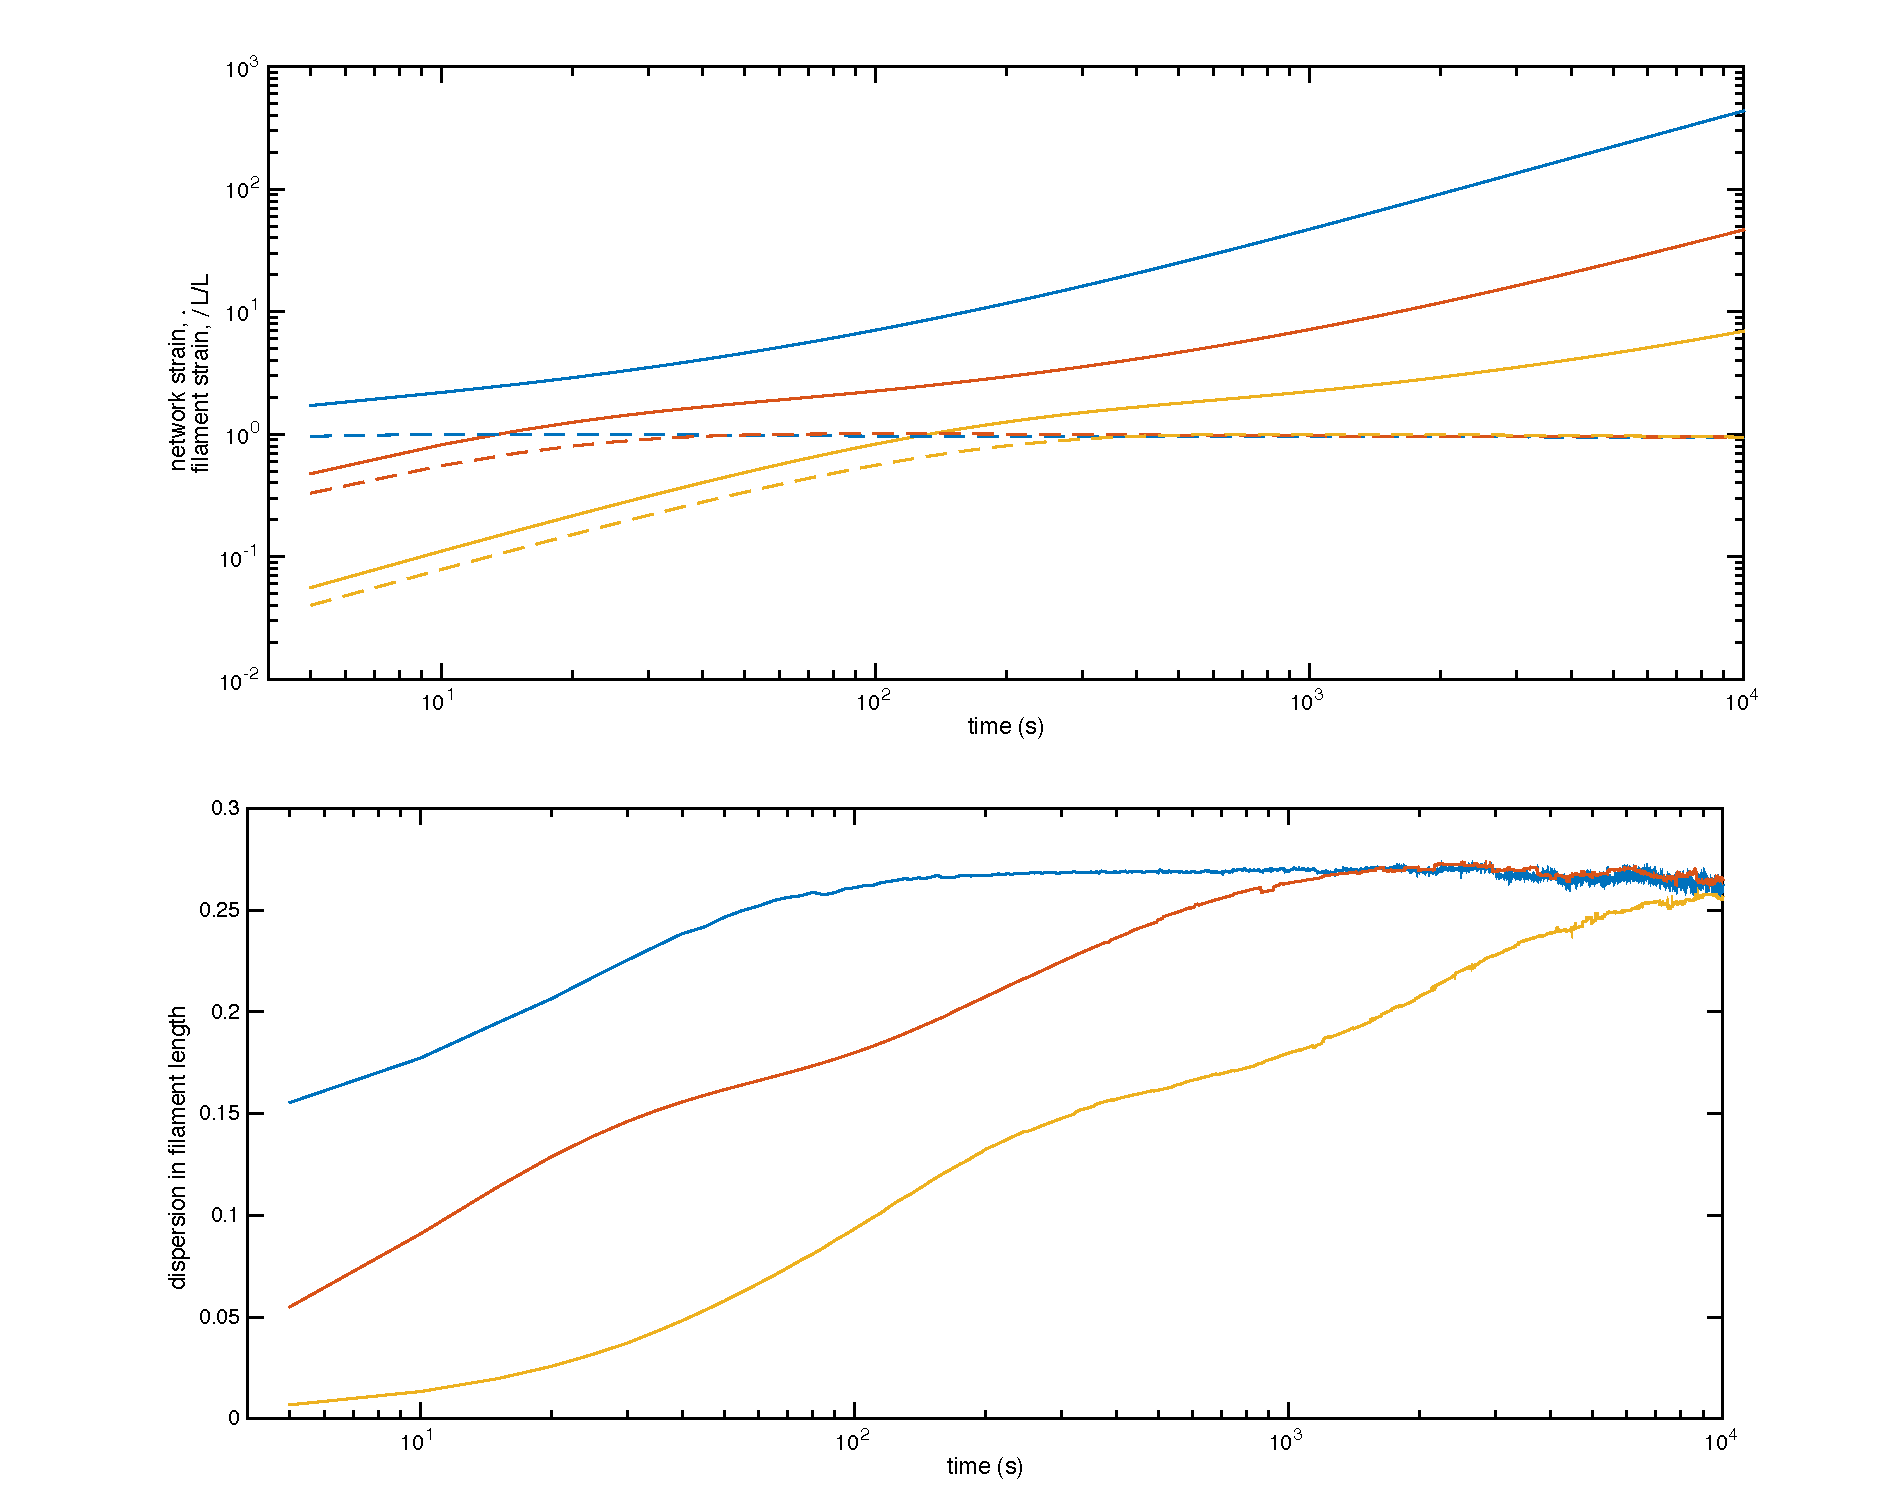
\includegraphics[width=\hsize]{glass_relax}
\caption{\label{fig:glass_relax} A. Creep response of networks and filament extension for different filament compliances.  B. Variation from mean filament extension for the networks in A. }
\end{figure}



Eventually the strain rate from slow filament stretching will become negligible compared to that due to pure cross-link slip on rigid rods.  This occurs on a timescale similar to that of cross-link slip and causes the effective viscosity to decay back toward the rigid limit.  This gives rise to a less-than-linear creep response during times after the initial elastic relaxation but before full filament relaxation from cross-link slip.   The transition begins to take place as the slip-derived strain reaches moves from 10 to 100 times the scale as that from pure mechanical stretching.  This feature is shown to be independent of the actual slip timescale that determines when this will occur in Figure \ref{fig:strain_coll}.

\begin{figure}[h!]
\centering
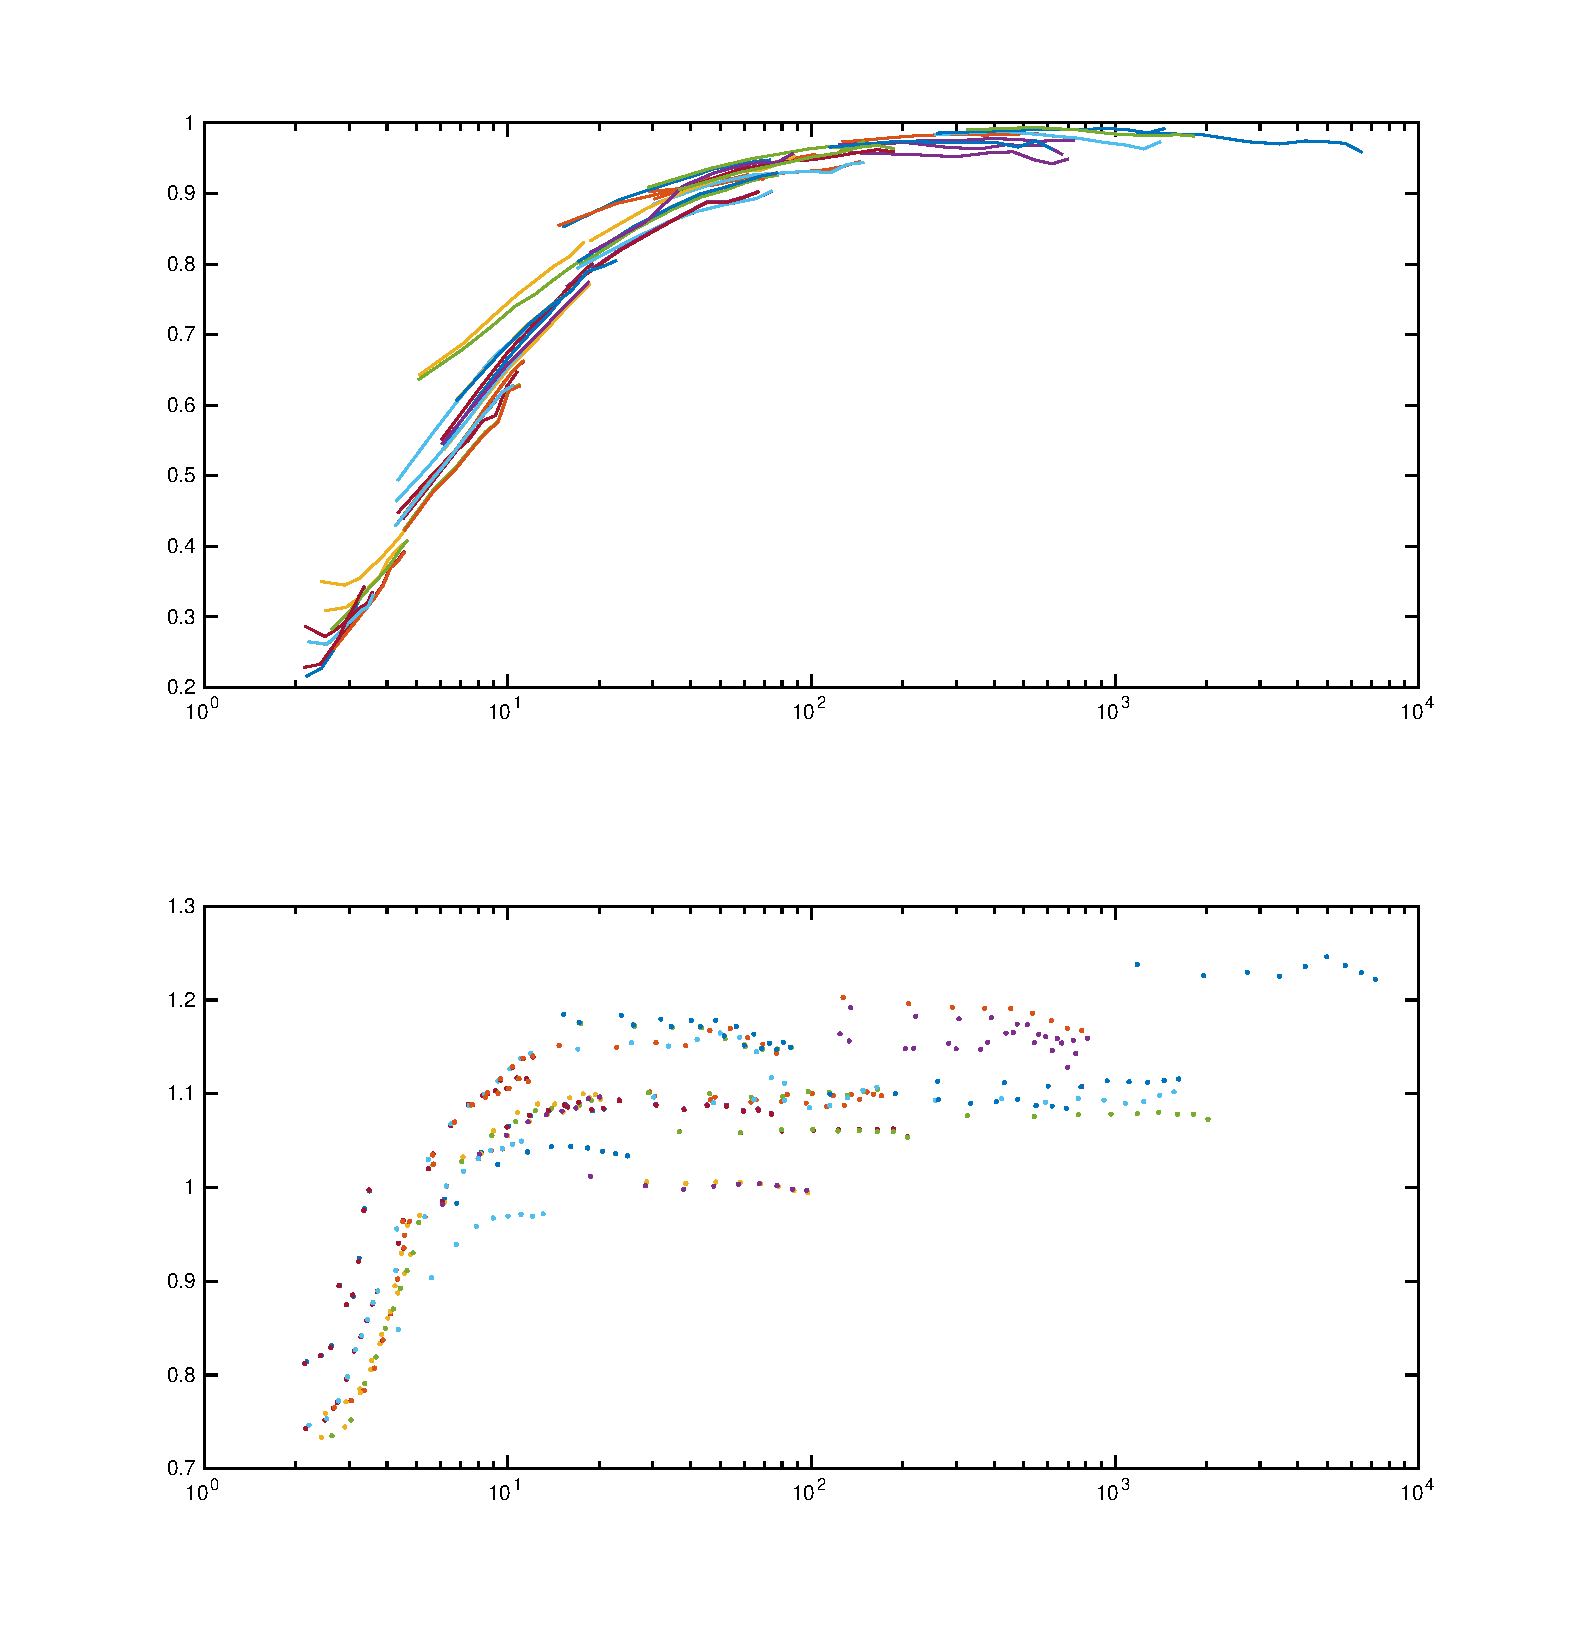
\includegraphics[width=\hsize]{strain_collapse}
\caption{\label{fig:strain_coll} A. Dependence of strain rate exponent as a function of strain relative to pure mechanical strain.  B.  Corresponding dispersion in filament strain, $\epsilon$, as a function of strain relative to pure mechanical strain. }
\end{figure}

\subsubsection{Phase D: Alignment at High Strain and Network Tearing}

Once the network is able to accumulate a large strain, the assumption of nearly uniform distributions of filament orientations begins to break down.

At this point the filament orientations become unevenly distributed $\langle \delta L / L \rangle \neq \gamma_{xy}sin(\theta)cos(\theta)$, with a larger number of filaments aligning in the direction of extension rather than compression.  Filament alignment, conceptually, causes the formation of subdomains that no longer span the space of the network. To the authors knowledge an exact derivation of the dependence of network connectedness on filament alignment has not been carried out, but Monte Carlo simulations have been used to show that alignment does indeed lead to lower connectedness\cite{model_percolationanisotropy}.

Although a lengthy discussion of this behavior would be valuable, we've found the computational cost of exploring these kinds of alignment tearing networks to be prohibitive in their study at this time.  Instead we now focus on just a few examples to garner some understanding.

\begin{figure}[h!]
\centering
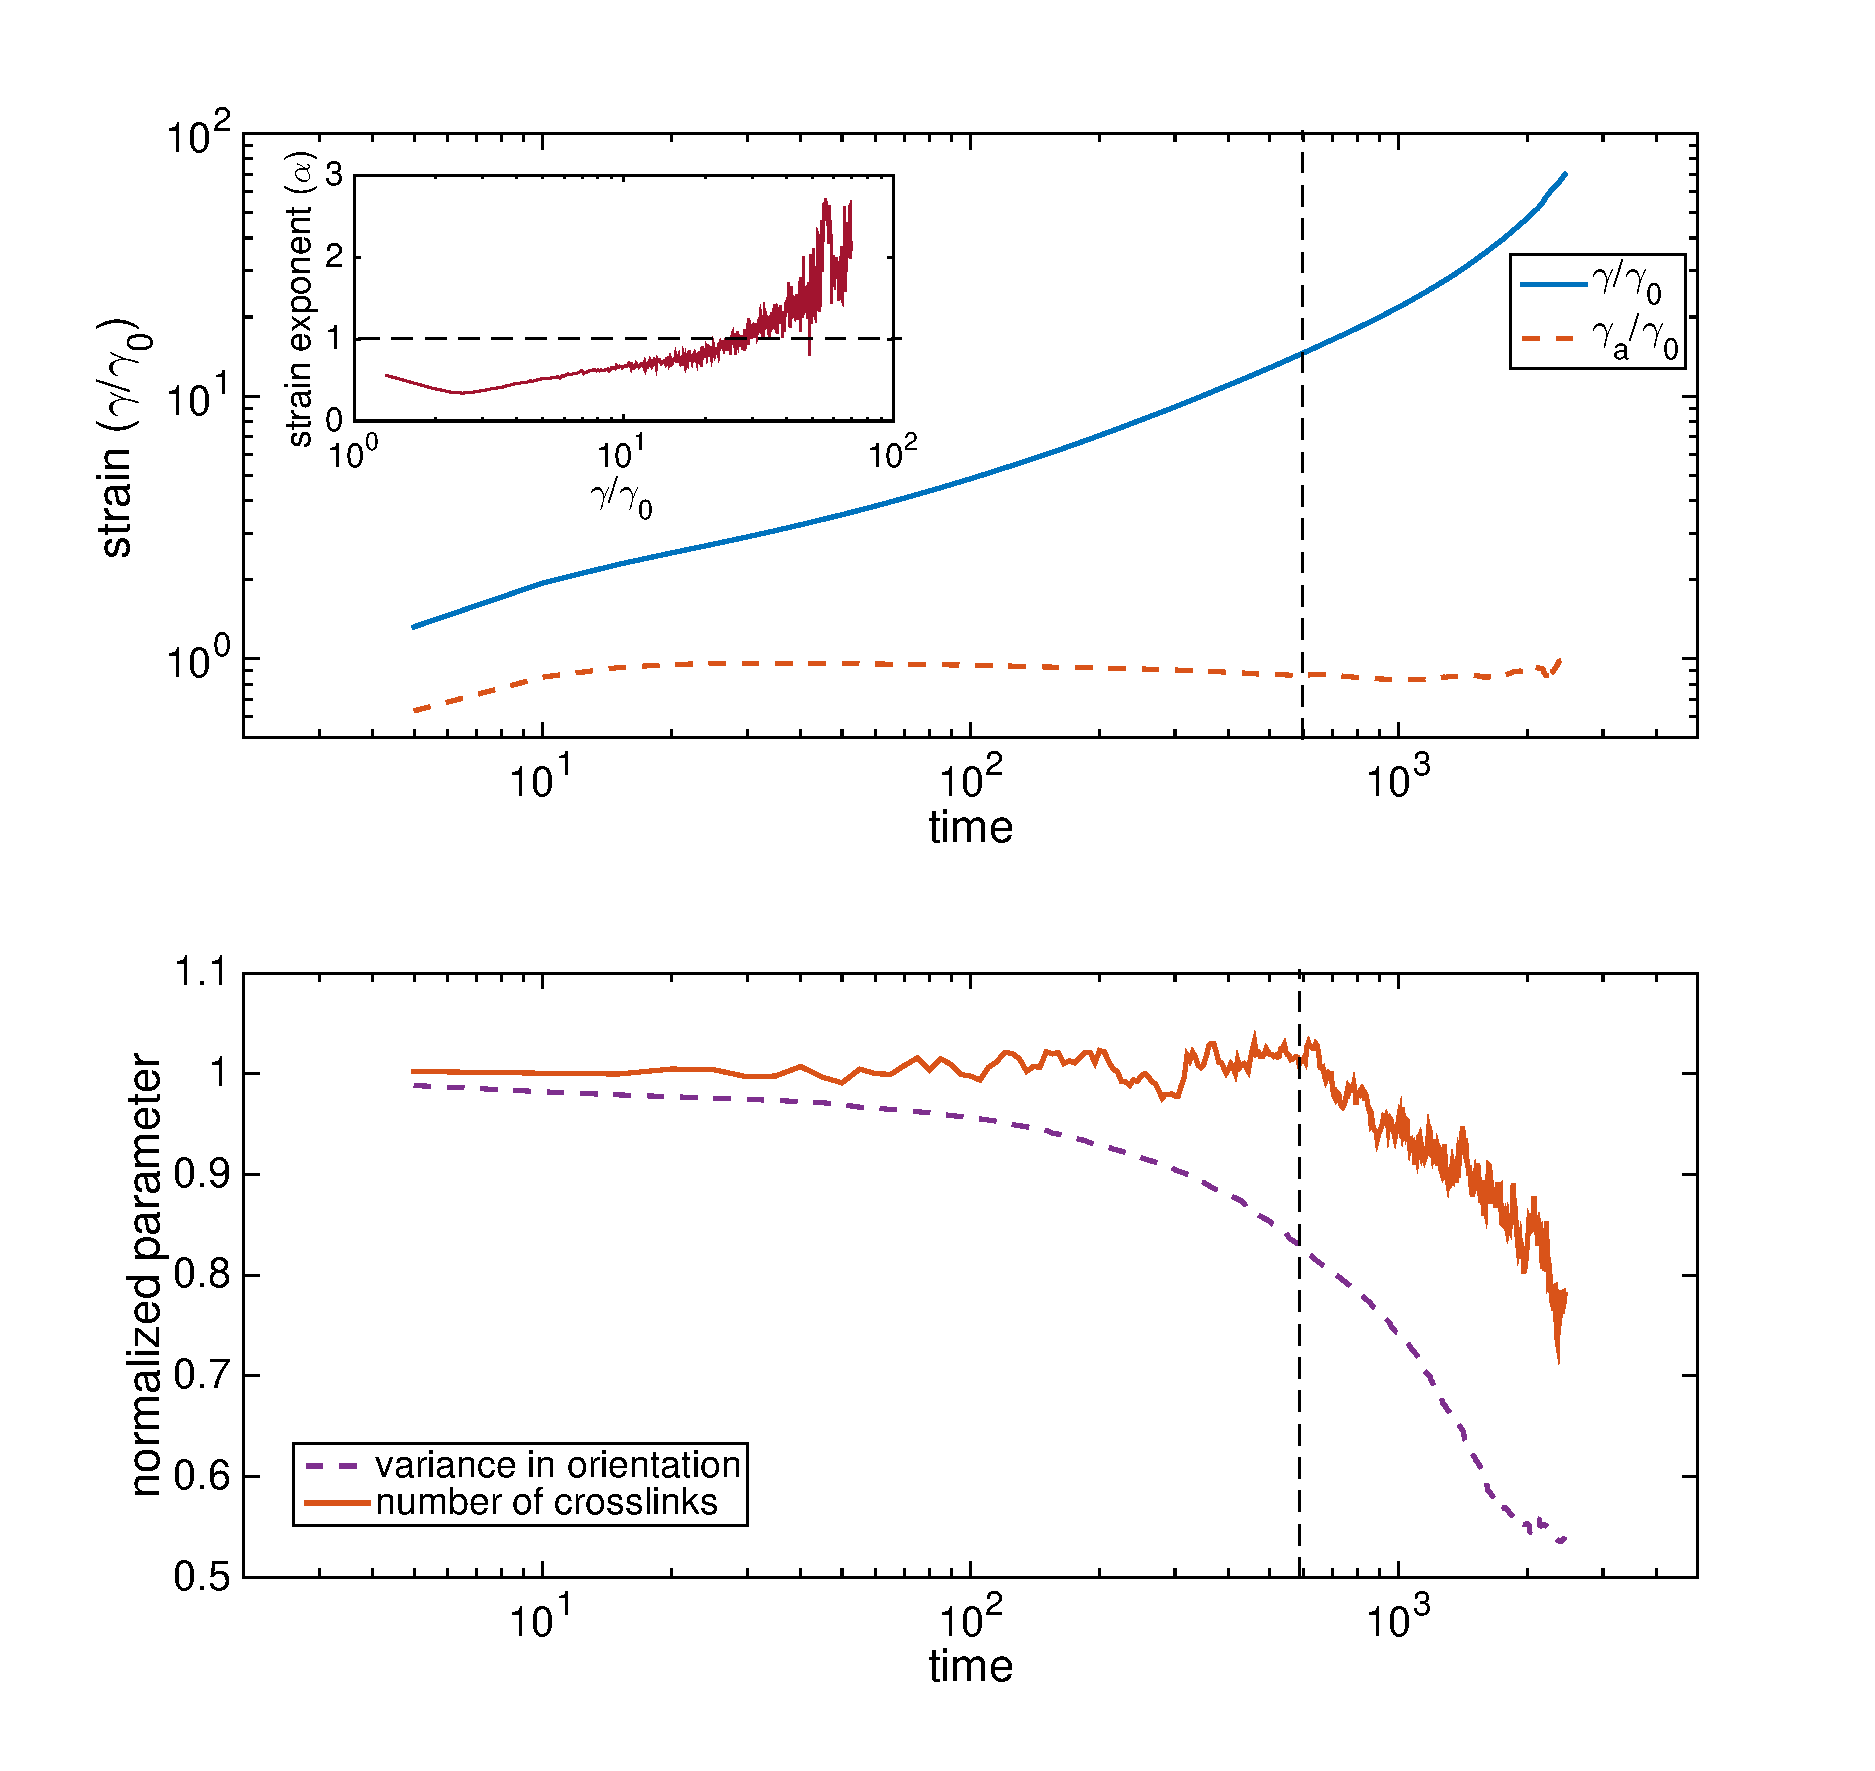
\includegraphics[width=\hsize]{tearer}
\caption{\label{fig:tearer} A. Creep response of a network transitioning to phase D. Inset shows strain exponent as a function of strain (exponent passes 1).  B.  Traces for the relative angular dispersion and relative number of cross links corresponding to the same simulation as part A. }
\end{figure}

We find that over time, the orientational distribution of the filaments begins to peak around 45 degrees as the large strain induces alignment.  In Figure \ref{fig:tearer}, we see that as the angular standard deviation falls, this reorientation eventually leads to be fewer bonds bridging the network perpendicular to the line of strain.  As this connectivity begins to noticeably decrease, the observed effective viscosity decreases as well, giving rise to supralinear creep.  From the inset of Figure \ref{fig:tearer} we can also see that the onset of phase D occurred before the network had completely reached phase C, leading to a rapid transition between sub-linear and super-linear creep response.  Finally, it should be noted that the end of this simulation resulted in the network tearing apart.  



\subsection{Phase Diagram of Dominant Behavior}
Finally, to explore the transitions between the various phases, we measured the creep response for a computationally tractable network ($L/l_c = 25$), as we varied the filament extensional modulus and the cross-link friction coefficient.  In Figure \ref{fig:phase_diag} , we can see the trends for the transitions between phases A, B, and C.  The line for the transition to D is still speculative at this time.

\begin{figure}[h!]
\centering
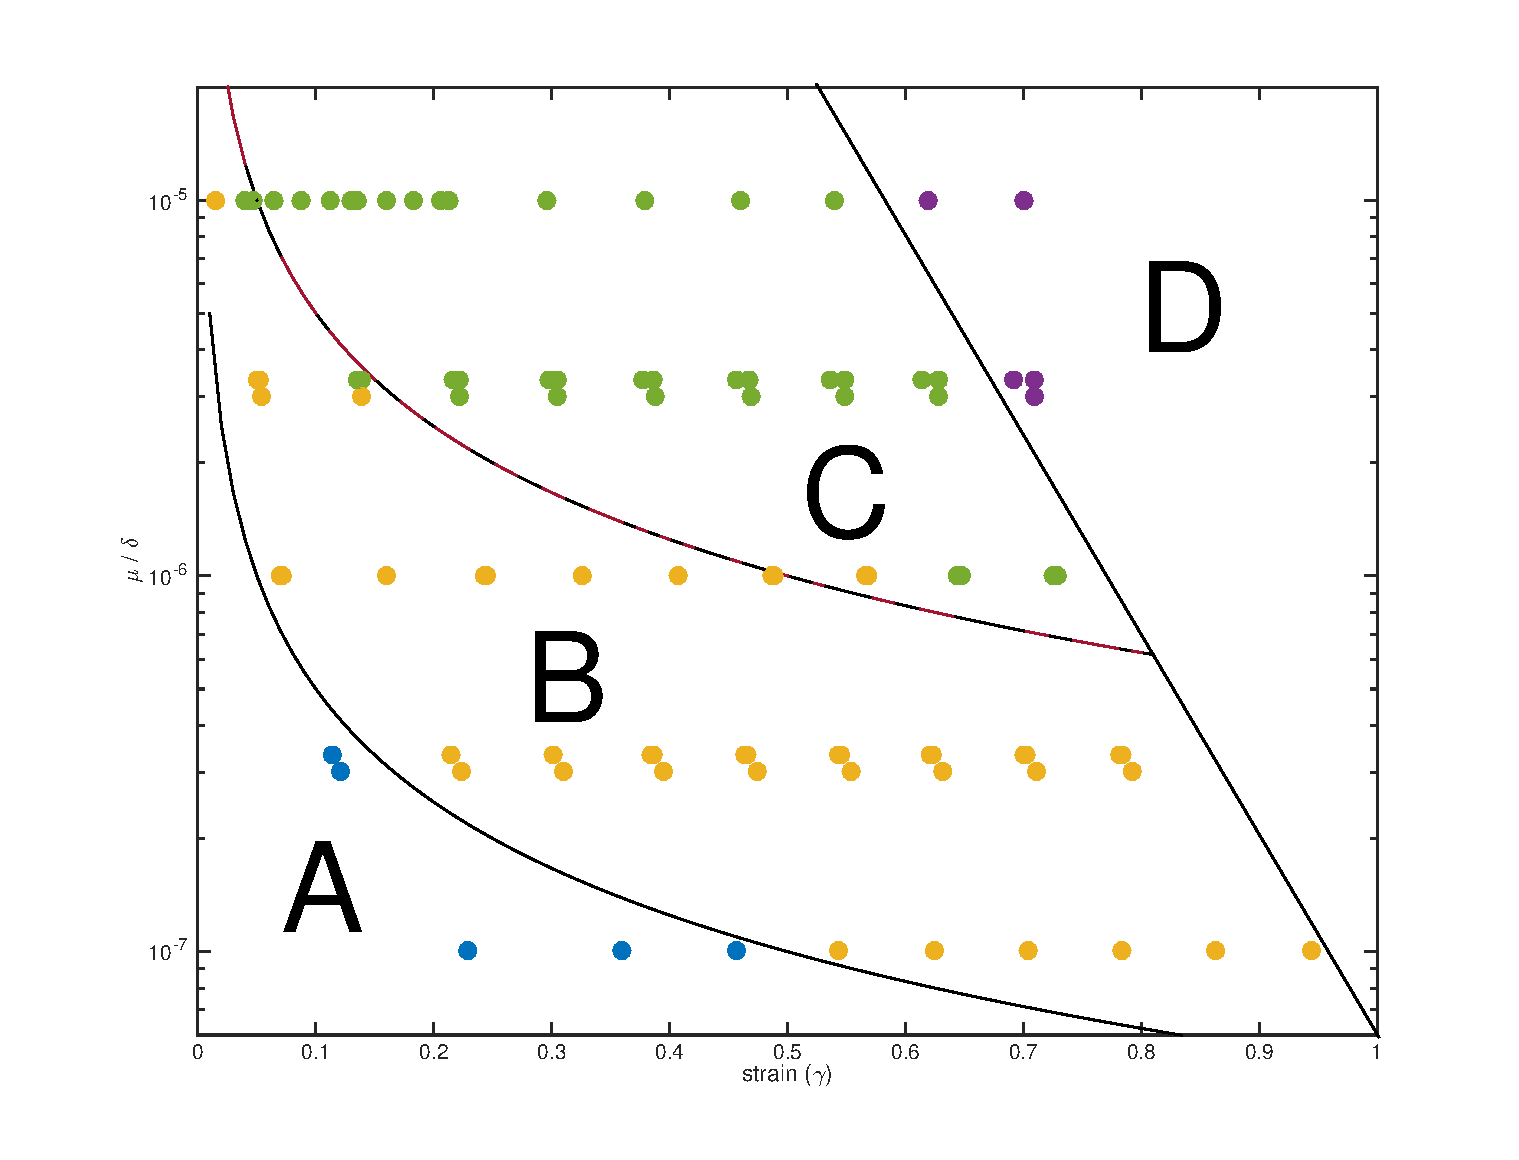
\includegraphics[width=\hsize]{phase_diag}
\caption{\label{fig:phase_diag} phase diagram of creep response for different filament extension, $\mu$ and cross-link friction, $\delta$.  Yellow, green, and purple dots correspond to creep measurements $\gamma \sim t^\alpha$ with $\alpha<0.92$, $0.92<\alpha<0.98$, or $\alpha>0.98$ respectively.  Blue dots represent creep measurements where $\gamma_{total} < 2\gamma_{mechanical}$}
\end{figure}


\subsection{Frequency dependent modulus}
This section will include a figure on the frequency dependent modulus once I get those.





















\section{Summary and Conclusions}
Conclusions I will draw after discussing the results with others.





















\section{Acknowledgements}
I'd like to thank Shiladitya Banerjee and Sayantan Majumdar for discussions on this topic.  Hopefully I can thank other people after I've spoken with them.

















\appendix
\addappheadtotoc




\section{Network Tearing under Extensional Stress}


\subsection{Extensional Thinning and Network Tearing}

For moderate extensional stresses, the rigid filament approximation of the effective viscosity simply picks up a different geometrical factor out front.  

However, at higher stress and in the presence of different things happen.

\begin{equation}
\frac{\partial l_c}{dt}=l_c\dot \gamma =\frac{l_c \sigma}{\eta}\sim l_c^3\frac{ \sigma}{L^2 \xi}
\end{equation}

We can see that the rate of network thinning accelerates as we would expect.  When the network reaches some minimum connectivity we assume that it stops behaving as a continuum material and the network tears irreversibly.  

\begin{equation}
\tau_{break} = \frac{\eta_{eff}}{2\sigma}\cdot\left ( 1 -\frac{l_c^2}{l_{break}^2} \right )
\end{equation}

This provides us with an estimate of the timescale of catastrophic breakdown for a network with a given initial architecture and molecular drag.


\subsection{Tearing Events During Extensional Strain}

This behavior is caused primarily by the low density network undergoing tearing events that interrupt global connectedness.  



\section{Nonlinear Extension and Long-Lived Strain Memory}

\subsection{Subnetwork Formation}

\subsection{Pull Release Simulations}

\subsection{Strain Memory}
Finally, we found an interesting behavior when we introduced non-linear extensional stiffness into our filaments.  This behavior mimics recent experiments in filamin cross-linked networks.  Filamin provides a high level of compliance to a network ($\gamma_0>0.5$) without substantial cross-link unbinding.  This allows large scale rearrangements to take place without driving very much cross-link slip, similar to the conditions in section \ref{sec:compliant}.  However, if we force individual filaments to undergo a strongly nonlinear stiffening at strains above 10\%, we find an interesting long term "strain storage."



For moderate strains, this result is largely the same as the result for extensional stress.  However, at larger deformations, extensional networks tear apart
To further explore the occurrence of tearing events ...


We explored a mode of deformation highly relevant to cortical mechanics in vivo.  Under this deformation stress was applied between a region of extension and region of compression.  Interestingly, until nearing the point of breakdown, the network did not experience a significant change in effective viscosity.  This was due to the between the diminishing viscosity of the thinning domain and the increasing viscosity of the thickening domain.  


Finally, we wished to explore the non-linear effects of reorientation of the filaments and non-linear network thinning/thickening.  To do so, we applied oscillatory shear 



\section{Deriving Molecular Drag Coefficients}
\label{app:drag}
Thus far, the idea of a molecular drag coefficient was taken as a phenomenological, measured parameter for a given experimental setup.  While this is a sufficient pragmatic justification, it's useful to try to motivate the quantitative value of this drag coefficient by connecting it to the underlying cross-link properties of binding affinity, concentration, and extensibility.

To do this we'll imagine the simplified case of two cross linkers sliding past each other in one dimension.  In this case, assume that we have an equilibrium number of bound cross-linkers, $n_B$, each of which is displaced from its equilibrium length by some distance $x$.  Each cross linker unbinds with rate $k_{off}$ and rebinds at it's relaxed position ($x=0$) with rate $k_{on}$.  At the same time, all the cross linkers are being pulled from their relaxed position at a rate, $v$, which is simply the rate at which the filaments are sliding past each other.  

We can right down an equation for the change in the density of cross-links at displacement $x$ as they are pulled upon, bind, and unbind.

\begin{equation}
\frac{\partial \rho}{\partial t} = -k_{off}\rho(x) - v\frac{\partial \rho}{\partial x} + k_{on}\delta(x)
\end{equation}

Recognizing that $\int \rho(x)=n_B$ implies $k_{on}=k_{off}n_B$, we can find the steady state solution

\begin{equation}
\rho(x) = \frac{n_b k_{off}}{v}\cdot exp\left ( -\frac{k_{off}}{v}x \right )
\end{equation}

If each cross-link has a spring constant $\mu_c$, then we can equate the force on all cross-links to the applied force that is sliding the filaments past each other.  Realistically, the spring constant and binding affinity would be functions of the cross-link stretch, but here we are taking them as approximately constant.  

\begin{equation}
\int_{0}^{\infty}\rho(x)\mu_cx dx = v \frac{\mu_c n_B}{k_{off}}= F_{app}
\end{equation}a

Therefore, the term next to v, (i.e. $\tfrac{\mu_c n_B}{k_{off}}$) would be equal to our molecular drag coefficient, $\xi$.  assuming, approximately 1-5 cross links per filament overlap, and using the following table of estimates pulled from Ferrer et al., we can chart the accuracy of this simple predictive model.

\begin{table}[h]
\begin{tabular}{| l | c | c |}
\hline
\textbf{cross-linker type} & $\alpha$-actinin & filamin-A  \\ \cline{1-1}
\textbf{dissociation constant ($s^{-1}$)} & 0.4 & 0.6 \\ \cline{1-1}
\textbf{spring constant ($nN / \mu m$)} & 455 & 820 \\ \cline{1-1}
\textbf{drag coefficient ($\tfrac{nN \cdot s}{\mu m}$)} & 200-1000 & 500-2500 \\ 
\hline
\end{tabular}
\end{table}



This molecular description assumed both a constant off-rate and linear force extension of cross-links.  In the event that binding kinetics are regulated by the state of extension, we would expect (based on Rf) to find a region that exhibits a stick-slip behavior instead of the smooth.  Depending on the nature of any coupling between cross-links local stick-slip could either give rise to a global stick-slip behavior or a heterogenous mixture of stuck and sliding cross-links.  It would be interesting to explore this topic further in the future, but in the present analysis, we choose to ignore complications from these nonlinear effects.

\section{Deriving Filament and Cross-Link Composite Extensional Modulus}
\label{app:compos}
Section describing how you derive the extensional modulus.


\begin{comment}
\section{Rigid Rod Approximation with Non-Uniform Distributions of Length and Orientation}
\label{app:aargh}
Section describing how you derive the extensional modulus.



\section{Semiflexibiliy}

Brief section showing that the results are not thoroughly flummoxed by semi flexibility.

\section{Simulation details}

All changes in the force felt by an endpoint are made smooth to allow integration of the differential equation (i.e. moving between stress domains, constraint domains, and overlap coupling occurs smoothly to prevent discontinuities).  Parameter conditions that cause instabilities are excluded, and the endpoint trajectories are integrated out to at least 1000 seconds. In addition, because we wish to probe the behavior of large scale network deformations, we are neglecting the sub-dominant effects from small thermal fluctuations. 


And I think I'll probably include all the gory details of how my simulations work since I'll be wanting to have direct references to the code. 
\begin{verbatim}
double y0 = 10; // example of declaration and assignment statement
double v0 = 0;  // initial velocity
double t = 0;   // time
double dt = 0.01; // time step
double y = y0; // solved all problems
\end{verbatim}
\end{comment}
\bibliographystyle{plain}
\bibliography{references}

\end{document}